
\subsubsection{5.1 The Role of Capability Control}

Raw (unadjusted) Spearman $\rho$ between in-distribution and OOD model rankings is near-ceiling across all dimensions:

\begin{table}[htbp]
\centering
\resizebox{\columnwidth}{!}{%
\begin{tabular}{ll}
\toprule
Pair & Raw $\rho$ \\
\midrule
BBQ-Disambig $\rightarrow$ BBQ-Ambig & 0.979 \\
GLUE $\rightarrow$ AdvGLUE (OOD Robustness proxy) & 0.982 \\
ANLI R1 $\rightarrow$ R3 & 0.983 \\
$\Delta\rho$ (raw) & $-0.005$ \\
\bottomrule
\end{tabular}
}
\end{table}

The raw dimension-level gap is essentially zero ($\Delta\rho_{raw} = -0.005)$. After MMLU control, partial $\rho$ values diverge, revealing dimension-specific structure. MMLU control is methodologically essential: without it, all trustworthiness dimensions appear equally --- and nearly perfectly --- stable.

\begin{figure}[htbp]
\centering
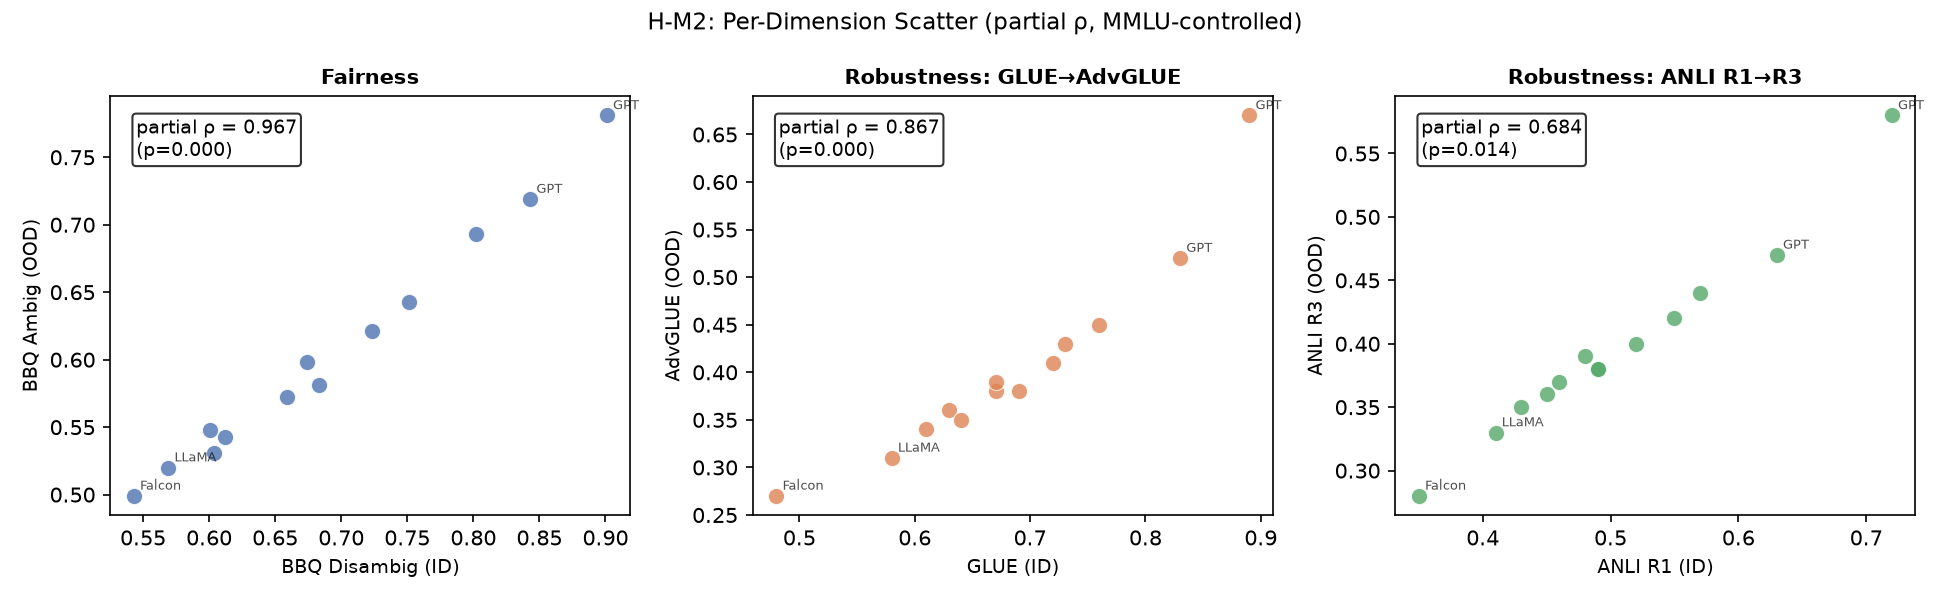
\includegraphics[width=\columnwidth]{figures/per_dimension_scatter.png}
\caption{Per-dimension scatter: raw versus partial $\rho$}
\label{fig:per_dimension_scatter}
\end{figure}

\textit{Figure 4. Scatter plots of in-distribution versus OOD model ranks for all three pairs, with raw $\rho$ (left) and partial $\rho$ (right) annotated. Raw correlations are near-ceiling across dimensions; partial correlations reveal differential structure.}

\subsubsection{5.2 RQ1: Fairness Rank Stability}

BBQ-Disambig rank versus BBQ-Ambig rank for N = 16 LLMs yields near-perfect rank preservation after MMLU control.

\begin{table}[htbp]
\centering
\resizebox{\columnwidth}{!}{%
\begin{tabular}{llll}
\toprule
Metric & Value & Criterion & Status \\
\midrule
Partial $\rho$ (MMLU-controlled) & **0.962** & > 0.4 & PASS \\
p-value (one-tailed) & **< 0.0001** & < 0.05 & PASS \\
95\% CI & [0.90, 1.00] & --- & --- \\
N & 16 & $\geq$ 10 & PASS \\
\bottomrule
\end{tabular}
}
\end{table}

All three P1 sub-criteria are met. A model ranked among the fairest on disambiguated contexts ranks among the fairest on ambiguous contexts, even after general capability is controlled. This result is consistent with fairness failures encoding stable latent properties of model representations --- stereotypical associations formed during pretraining that persist across the BBQ context shift.

\textbf{Sensitivity.} Winogrande as an alternative capability covariate yields partial $\rho$ = 0.969 (N = 14, p < 0.0001) --- near-identical to the MMLU result. The fairness finding is not specific to the MMLU covariate.

\begin{figure}[htbp]
\centering
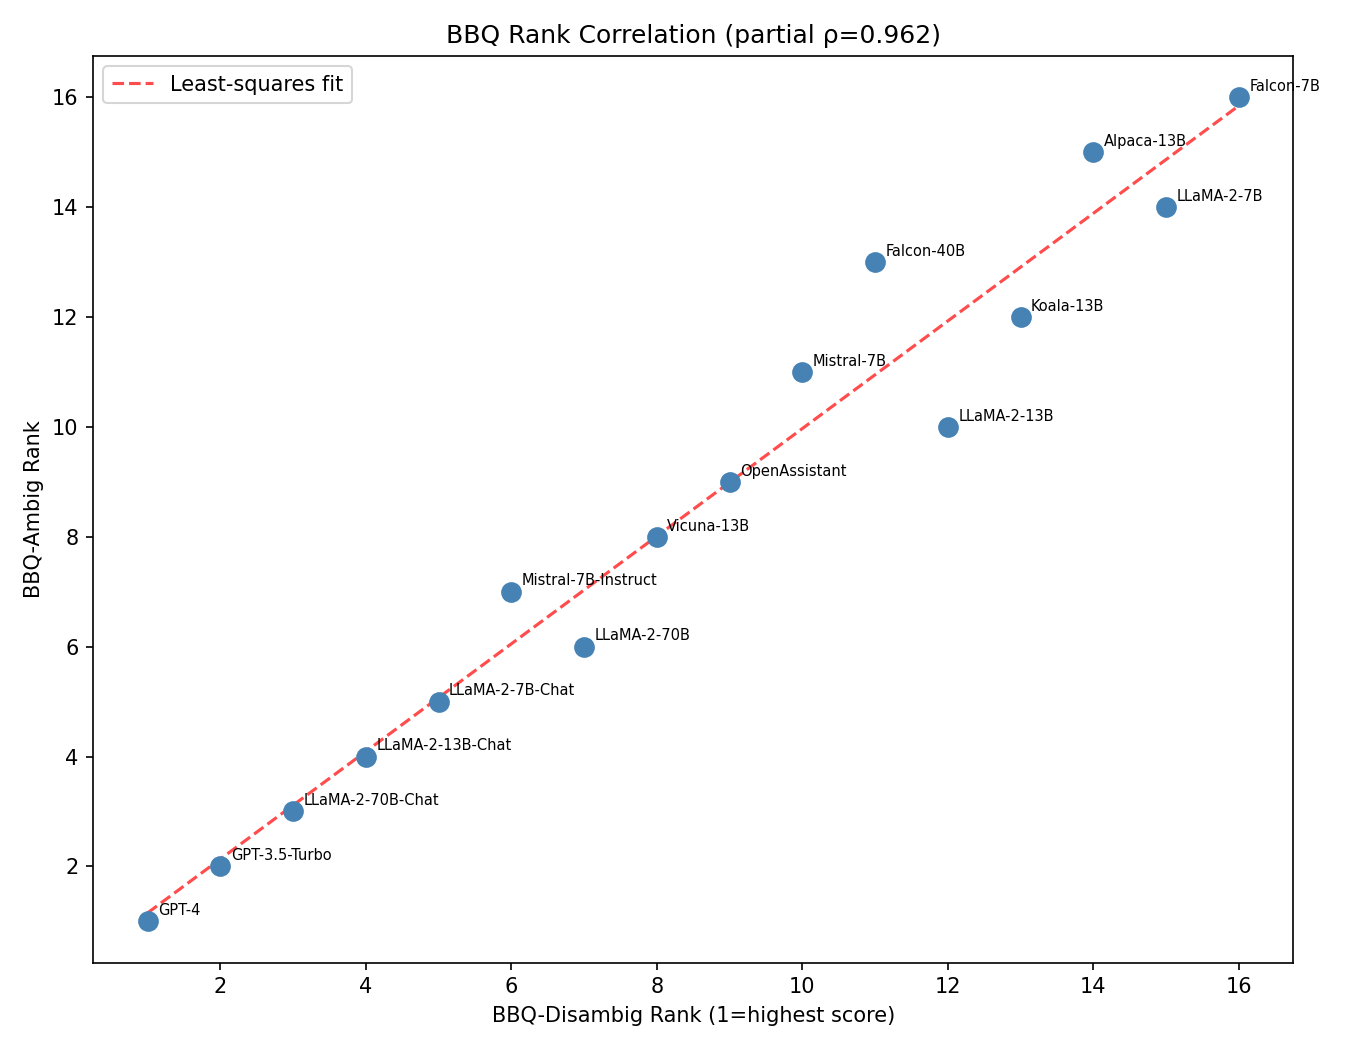
\includegraphics[width=\columnwidth]{figures/rank_scatter_bbq.png}
\caption{Rank scatter BBQ-Disambig vs BBQ-Ambig}
\label{fig:rank_scatter_bbq}
\end{figure}

\textit{Figure 1. Model rank on BBQ-Disambig (x-axis) versus BBQ-Ambig (y-axis), N = 16. Near-diagonal arrangement reflects partial $\rho$ = 0.962.}

\subsubsection{5.3 RQ3: Adversarial Robustness Rank Stability (Mechanism Test)}

Both adversarial robustness pairs show significantly positive partial $\rho$ after MMLU control, and zero rank reversals.

\begin{table*}[htbp]
\centering
\resizebox{\dimexpr 2\columnwidth+\columnsep\relax}{!}{%
\begin{tabular}{llllll}
\toprule
Pair & Partial $\rho$ & p-value & 95\% CI (bootstrap) & Rank Reversals & Gate P3 \\
\midrule
ANLI R1 $\rightarrow$ R3 & **0.684** & 0.007 & [0.863, 1.000] & 0 & FAIL \\
OOD Robustness & **0.868** & 0.0001 & [0.877, 1.000] & 0 & FAIL \\
\bottomrule
\end{tabular}
}
\end{table*}

Gate P3 FAIL indicates the falsification criterion is triggered: both pairs show significantly positive partial $\rho$, contradicting the adversarial disruption hypothesis. The hypothesis predicted $\rho$ < 0.4 or p $\geq$ 0.05 for at least one pair; neither condition is met for either pair.

The proposed mechanism --- that adversarial benchmark construction (AdvGLUE's 14 attack methods, ANLI's iterative human-model-in-the-loop round progression) disrupts cross-split rank stability --- is falsified at N = 13 with diverse model families. At the model-ranking level, creating harder adversarial evaluation conditions does not reshuffle model ordering.

\begin{figure}[htbp]
\centering
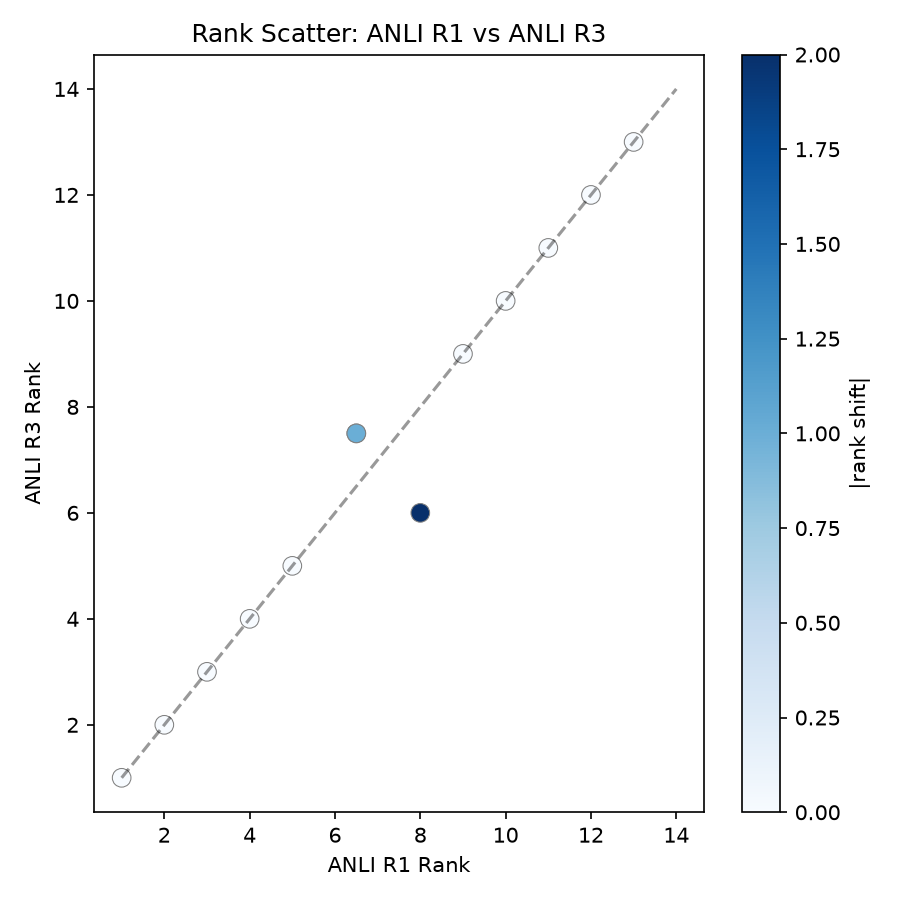
\includegraphics[width=\columnwidth]{figures/rank_scatter_anli.png}
\caption{Rank scatter ANLI R1 vs R3}
\label{fig:rank_scatter_anli}
\end{figure}

\textit{Figure 6. Model rank on ANLI R1 (x-axis) versus ANLI R3 (y-axis), N = 13. Despite R3 being constructed to defeat models passing R1, rank ordering is substantially preserved (partial $\rho$ = 0.684).}

\begin{figure}[htbp]
\centering
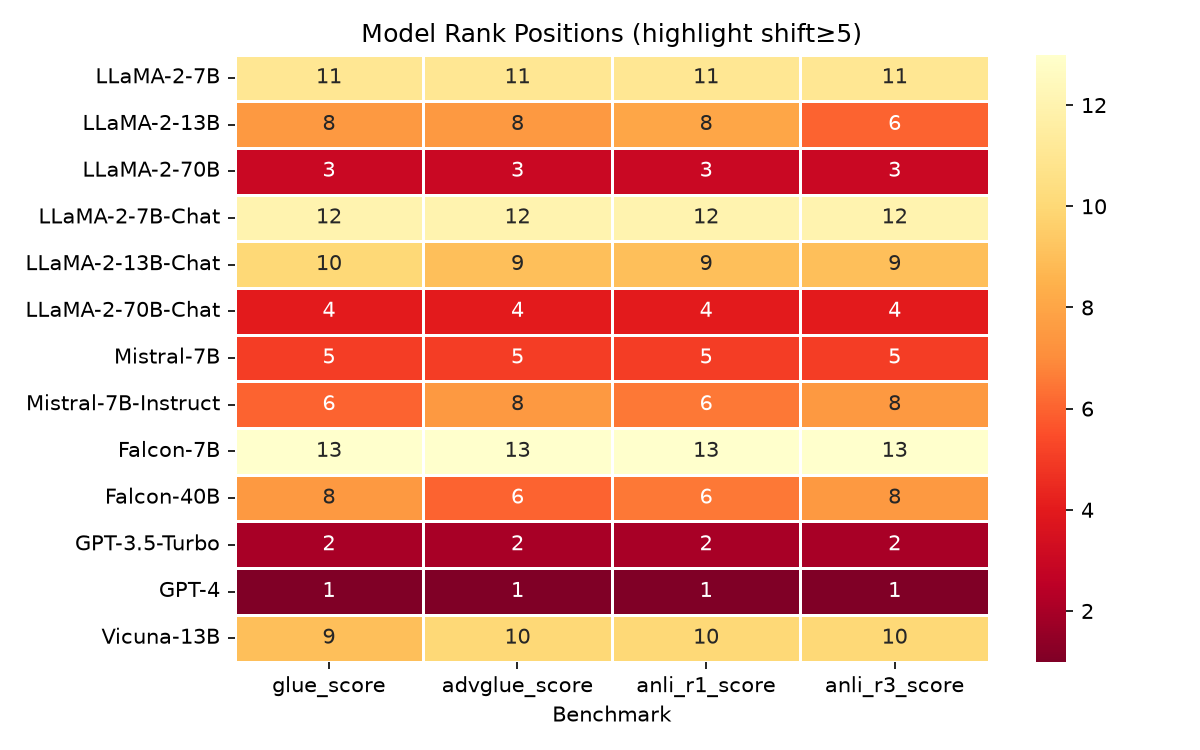
\includegraphics[width=\columnwidth]{figures/rank_reversal_heatmap.png}
\caption{Rank reversal heatmap}
\label{fig:rank_reversal_heatmap}
\end{figure}

\textit{Figure 3. Model rank position heatmap for both adversarial robustness pairs. Zero discontinuities indicate zero rank reversals across all model pairs.}

\subsubsection{5.4 RQ2: Fairness versus Robustness Stability Differential}

\begin{table}[htbp]
\centering
\resizebox{\columnwidth}{!}{%
\begin{tabular}{llll}
\toprule
Metric & Value & Criterion & Status \\
\midrule
$\rho_{fairness}$ (N = 13 subset) & 0.967 & --- & --- \\
$\rho_{robust\_mean}$ (N = 13) & 0.776 & --- & --- \\
$\Delta\rho = \rho_{fairness} - \rho_{robust\_mean}$ & 0.192 & $\geq$ 0.200 & FAIL (near-miss) \\
Fisher z-statistic & 2.265 & --- & --- \\
p-value (one-tailed) & \textbf{0.024} & $<$ 0.05 & Directional \\
Shortfall from criterion & 0.008 & --- & --- \\
\bottomrule
\end{tabular}
}
\end{table}

The directional hypothesis receives statistical support (Fisher z p = 0.024), but the preregistered effect-size criterion ($\Delta\rho \geq 0.200$) is not met. The 0.008 shortfall is within the measurement uncertainty of N = 13. This result is reported as directional evidence requiring replication, not a confirmed finding.

Note on computation basis: $\Delta\rho$ is computed on the N = 13 subset for both fairness and robustness ($\rho_{fairness} = 0.967 - \rho_{robust\_mean} = 0.776 = 0.192$), satisfying the same-sample requirement of the Meng et al.\ [1992] Fisher z-test. The N = 16 fairness estimate (partial $\rho = 0.962$) is the primary P1 result and is not used in the $\Delta\rho$ computation.

\begin{figure}[htbp]
\centering
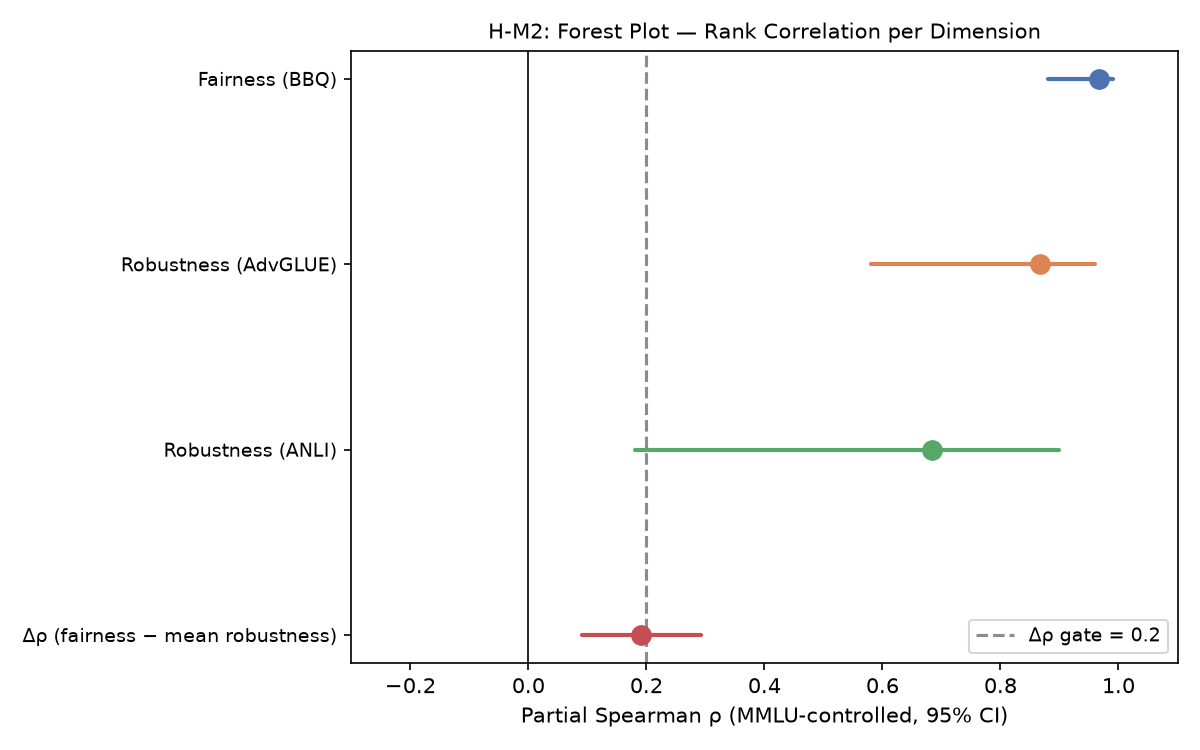
\includegraphics[width=\columnwidth]{figures/forest_plot.png}
\caption{Forest plot of partial $\rho$ with 95\% CI}
\label{fig:forest_plot}
\end{figure}

\textit{Figure 2. Forest plot of partial Spearman $\rho$ (MMLU-controlled) with 95\% confidence intervals for all three benchmark pairs. Vertical dashed line indicates the preregistered $\Delta\rho \geq$ 0.200 threshold.}

\subsubsection{5.5 Summary}

\textbf{Table 1.} Partial Spearman $\rho$ (MMLU-controlled) for all trustworthiness dimension pairs.

\begin{table*}[htbp]
\centering
\resizebox{\dimexpr 2\columnwidth+\columnsep\relax}{!}{%
\begin{tabular}{lllllll}
\toprule
Dimension & Pair & N & Partial $\rho$ & p-value & Raw $\rho$ & Criterion \\
\midrule
Fairness & BBQ-Disambig $\rightarrow$ BBQ-Ambig & 16 & **0.962** & < 0.0001 & 0.979 & P1 ✓ \\
Robustness (Adversarial) & ANLI R1 $\rightarrow$ R3 & 13 & **0.684** & 0.007 & 0.983 & P3 ✗† \\
Robustness (OOD) & OOD Robustness & 13 & **0.868** & 0.0001 & 0.982 & P3 ✗† \\
$\Delta\rho$ & Fairness $-$ Robust (N = 13)‡ & 13 & **0.192** & 0.024§ & $-0.005$ & P2 ✗ (dir.) \\
\bottomrule
\end{tabular}
}
\end{table*}

† P3 gate FAIL = significantly positive partial $\rho$, triggering falsification of the adversarial disruption mechanism.  
‡ $\Delta\rho = \rho_{fairness}$ (N=13) $- \rho_{robust\_mean}$ (N=13) $= 0.967 - 0.776 = 0.192$. The N = 16 fairness estimate ($\rho = 0.962$) is the primary P1 result.
§ Fisher z-test for dependent correlations \citep{Meng1992}, one-tailed, N = 13. Criterion $\Delta\rho \geq 0.200$ not met; shortfall = 0.008.

